\chapter{a title for chapter 1}
\label{chapter:chapter_1}
 
\section{section 1}
\label{section:section_1}

This is content.

\subsection{time}

A few time representations follow:

\begin{itemize}
\item \timeA\today
\item \timeB\today
\item \timeC\today
\item \timeD
\item \timeE
\item \timeF\today
\item \timeG\today
\end{itemize}

\subsection{units and units typesetting}

\begin{itemize}
\item \mathunit{${a^{b}}$}{m^{2}} -- correct unit typesetting (manual siunitx function) (preferred for mathematics mode, though note that the function for this is provided by aqueous [see below for manual equivalent method not dependent on aqueous])
\item \SI{10}{kg} -- correct unit typesetting (siunitx)
\item ${10\,\textnormal{kg}}$ -- incorrect unit typesetting (mathematics, textnormal)
\item 10 kg -- incorrect unit typesetting (literally)
\item \SI{10}{kg m s^{-2}} -- correct unit typesetting (siunitx)
\item ${10^{-28}}$\,\si{m^{2}} -- correct unit typesetting, though very manual (siunitx)
\item ${a^{b}}$\,\si{m^{2}} -- correct unit typesetting, though manual (siunitx) (preferred for mathematics mode)
\item \SI[parse-numbers=false]{a^{b}}{m^{2}} -- dodgy, manual correct unit typesetting (siunitx)
\item \SI[parse-numbers=false, number-math-rm=\ensuremath]{a^{b}}{m^{2}} (siunitx)
\end{itemize}

\begin{itemize}
\item The angle is ${14\degree}$.
\item The temperature is \SI{14}{\celsius}. -- correct unit typesetting (siunitx)
\end{itemize}

\subsection{mathematics}

The following is a referenced equation:

\begin{equation}
\label{equation:emc2}
E=mc^{2}
\end{equation}

This is a reference to equation \ref{equation:emc2}.

This is bold mathematics: ${t\bar{t}\bm{H}\left(b\bar{b}\right)}$.

This is bold mathematics: ${\bm{t\bar{t}H\left(b\bar{b}\right)}}$.

\subsection{lists}

This is a list:

\begin{itemize}
\item function,
\item Job,
\item JobGroup,
\item ParallelJobProcessor and
\item pool.
\end{itemize}

\newpage

This is a checklist:

\begin{description}
\item[\Checkmark] item
\item[\Checkmark] item
    \begin{description}
    \item[\Checkmark] subitem
    \item[\Checkmark] subitem
        \begin{description}
        \item[\Checkmark] subitem
        \end{description}
    \end{description}
\item[\Checkmark] item
\item[\XSolidBrush] item
\end{description}

\subsection{code}

This is some code:

\begin{center}
\footnotesize\texttt{Reco\_tf.py --inputBSFile data12.1234.RAW --outputESDFile data12.1234.ESD}
\end{center}

\subsection{images}

This is a figure set to a defined width:

\begin{figure}[H]
\begin{center}
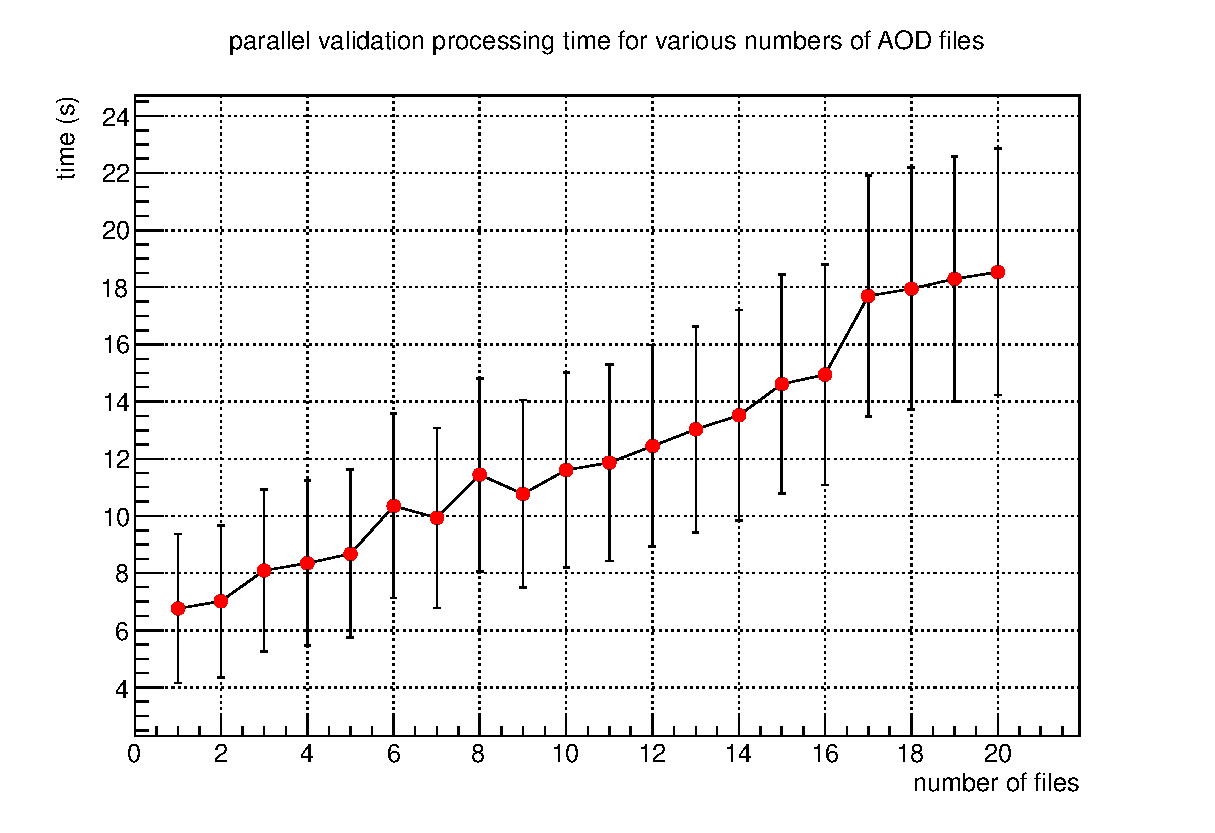
\includegraphics[width=\measureUSpecification]{images/2014-04-10_1.eps}
\end{center}
\caption{parallel job processor: large efficiency improvement as a result of parallelisation}
\end{figure}

This is a figure set to the text width:

\begin{figure}[H]
\begin{center}
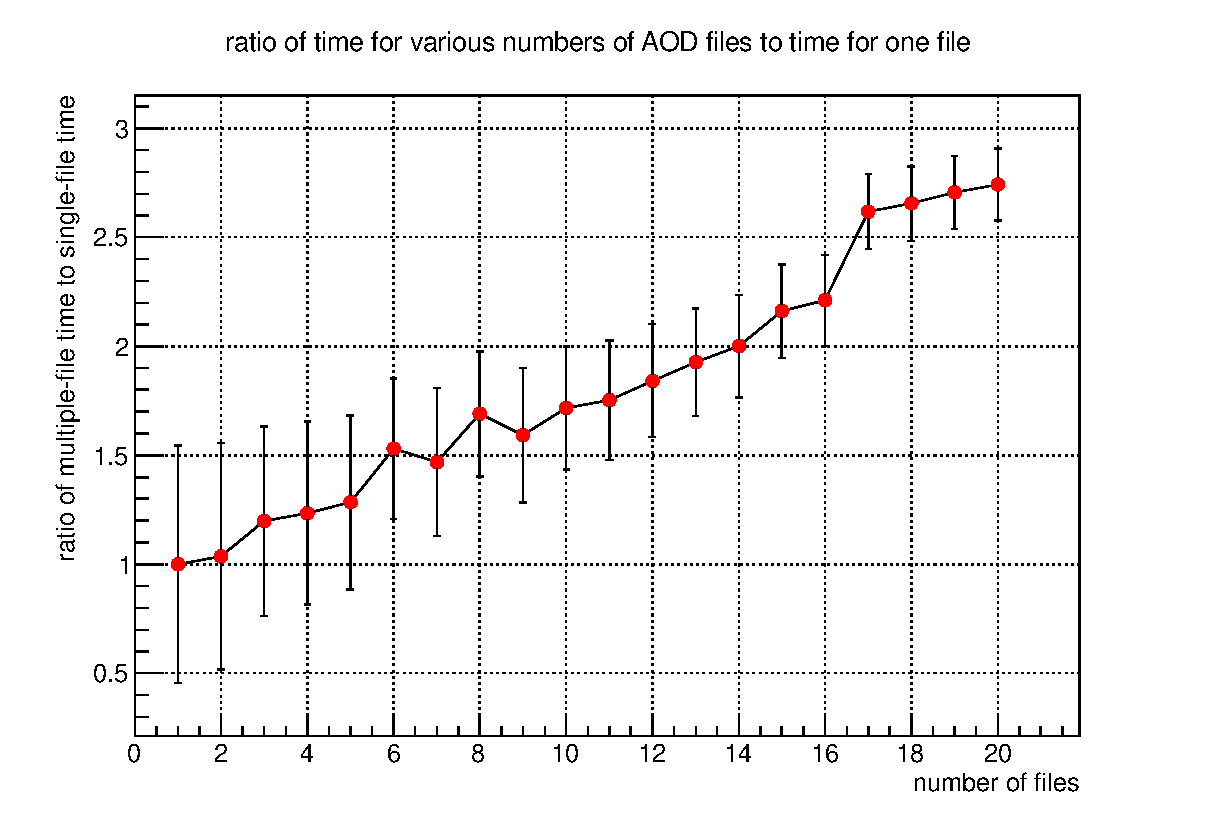
\includegraphics[width=\textwidth]{images/2014-04-10_2.eps}
\end{center}
\caption{parallel job processor}
\label{figure:PJP_1}
\end{figure}

\subsection{references}

This is a reference to figure~\ref{figure:PJP_1}. This is a reference~\cite{Tianjun_1}. This is another reference~\cite{McCulloch_Pitts_1}. This is a URL: \href{https://github.com/wdbm/aqueous}{\textcolor{black!100}{https://github.com/wdbm/aqueous}}

\cofeDm{0.4}{0.1}{90}{1 cm}{-7 cm}

\subsection{ROOT}

ROOT~\cite{ROOT} is an object oriented data analysis framework aimed at solving data analysis challenges in high energy physics. While \emph{ROOT} is simply a name, a possible acronym for the system could be \emph{``Rapid Object-Oriented Technology''}~\cite{ROOT_acronym}. ROOT was developed in the context of the NA49 experiment at CERN. NA49 generated data of approximately \mathunit{10}{TB} per run. This rate of data provided a test environment for the development of ROOT, as the next generation of data analysis. ROOT features \emph{Cling}, a C++ interpreter.\footnote{This is a footnote.}

\newpage

\subsection{some paragraphs}

\lipsum[1-4]

\newpage

\subsection{tables}

\begin{figure}[h]
\begin{center}
%\begin{table}[h]
\scriptsize
\begin{tabular}{p{3 cm}p{7 cm}}
\hline\hline
input file option&description\\
\hline
\texttt{--inputHitsFile}&input only\\
\texttt{--inputBSFile}&RAW data (BS = ByteStream), currently input only\\
\texttt{--inputRDOFile}&\\
\texttt{--inputESDFile}&\\
\texttt{--inputAODFile}&\\
\hline\hline
\end{tabular}
%\end{table}
\end{center}
\mbox{}\newline
\begin{center}
%\begin{table}[h]
\scriptsize
\begin{tabular}{p{3 cm}p{7 cm}}
\hline\hline
output file option&description\\
\hline
\texttt{--outputRDOFile	valid}&if starting from Hits\\
\texttt{--outputESDFile	valid}&if starting from Hits, RDO or BS\\
\texttt{--outputAODFile	valid}&if starting from ESD or anything else upstream\\
\texttt{--outputNTUP\_XXXFile}&can be made from ESD or AOD, BS or RDO\\
\hline\hline
\end{tabular}
%\end{table}
\end{center}
\caption{Reco\_tf.py usage}
\end{figure}
